
\documentclass[tikz,border=10pt]{standalone}
\begin{document}
    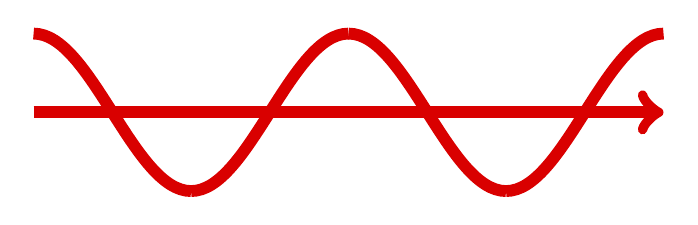
\begin{tikzpicture}
    \draw[ultra thick, color=black!15!red,line width=1.5mm,->] (4,0) -- (12,0);
    \draw[ultra thick, color=black!15!red,line width=1.5mm] (4,1) cos (5,0);
    \draw[ultra thick, color=black!15!red,line width=1.5mm] (5,0) sin (6,-1);
    \draw[ultra thick, color=black!15!red,line width=1.5mm] (6,-1) cos (7,0);
    \draw[ultra thick, color=black!15!red,line width=1.5mm] (7,0)  sin (8,1);
    \draw[ultra thick, color=black!15!red,line width=1.5mm] (8,1) cos (9,0);
    \draw[ultra thick, color=black!15!red,line width=1.5mm] (9,0) sin (10,-1);
    \draw[ultra thick, color=black!15!red,line width=1.5mm] (10,-1) cos (11,0);
    \draw[ultra thick, color=black!15!red,line width=1.5mm] (11,0) sin (12,1);
    \end{tikzpicture}

\end{document}
